\chapter{CSV Definition}
\label{ap:csv}
The wind farm data is of the file type csv. The file can be split up into 2 pieces.
\section{The header}
The header consists of two lines. The first line defines the latitude, longitude and the name of the wind farm from which the data originates.
The second line defines the columns, which \textbf{has} to be the same as shown in listing \ref{ap:ex:csv}.

\section{The body}
The third and following lines contains the data itself.

\section{Template}
\lstinputlisting[language=sql,caption={CSV template},label=ap:ex:csv]{./appendix/template.csv}

\chapter{Use cases}
\label{ap:usecase}
We have two types of actor:
\begin{itemize}
\item User: Ordinary person.
\item Admin: User with permission to access administration.
\end{itemize}

\section{Clicking on a radar at the map}
\textbf{Actor:} User

\textbf{Scenario:}
\begin{itemize}
\item Checks if there is data for the date
\item If images isn't generated, it will generate them real time.
\item Radar shows images over an interval.
\item \emph{One click for play/pause and doubleclick for reset.}
\item When there is no more data, the radar resets.
\end{itemize}
\textbf{Alternative scenario:} 
\begin{enumerate}
\item No data is available for that moment and a message appears.
\end{enumerate}

\section{Clicking on a wind farm at the map}
\textbf{Actor:} User

\textbf{Scenario:}
\begin{itemize}
\item Visualize data for that given wind farm.
\end{itemize}

\section{Changing view in chart for wind farm}
\textbf{Actor:} User

\textbf{Scenario:}
\begin{enumerate}
\item Changing to 2-week view.
\begin{itemize}
\item Changing chart view interval to 2 weeks.
\item Load new data for the new interval.
\end{itemize}
\item Changing to weekly view.
\begin{itemize}
\item Changing chart view interval to 1 week.
\item Load new data for the new interval.
\end{itemize}
\item Changing to daily view.
\begin{itemize}
\item Changing chart view interval to 1 day.
\item Load new data for the new interval.
\end{itemize}
\end{enumerate}

\section{Changing data to be shown}
\textbf{Actor:} User

\textbf{Scenario:}
\begin{itemize}
\item The data is shown.
\end{itemize}
\textbf{Alternative scenario}
\begin{enumerate}
\item The data is removed.
\end{enumerate}

\section{Using control buttons in chart for wind farm}
\textbf{Actor:} User

\textbf{Scenario:}
\begin{enumerate}
\item Pressing fast backward.
\begin{itemize}
\item Go two weeks back on 2-week view, one week back on weekly view and one day on daily view.
\item Loads new data.
\end{itemize}
\item Pressing backward.
\begin{itemize}
\item Go one week back on 2-week view, one day back on weekly view and one hour on daily view.
\item Loads new data.
\end{itemize}
\item Pressing play.
\begin{itemize}
\item Change to daily view and go one hour forward every second.
\item Loads new data.
\end{itemize}
\item Pressing forward.
\begin{itemize}
\item Go one week forward on 2-week view, one day forward on weekly view and one hour on daily view.
\item Loads new data.
\end{itemize}
\item Pressing fast forward.
\begin{itemize}
\item Go two weeks forward on 2-week view, one week forward on weekly view and one day on daily view.
\item Loads new data.
\end{itemize}
\end{enumerate}

\section{Upload file}
\textbf{Actor:} Admin

\textbf{Scenario:}
\begin{itemize}
\item Sign in with correct username and password.
\item Add new file (CSV, WRK, ZIP) and enter correct timezone.
\item If file is ZIP, it will decompress.
\item File is uploaded.
\item File is being parsed.
\end{itemize}
\textbf{Alternative scenario:} 
\begin{enumerate}
\item Sign in with wrong username or password.
\item Adding file that isn't correct format and get an error message.
\item Adding ZIP file, but files inside zip isn't correct. It will get an error message.
\item File exists and will not be uploaded.
\end{enumerate}

\chapter{Installation}
\label{ap:installation}
\chapter{Installation}

In the following it is implied that the chosen solutions for each step - e.g. if more than one option is possible - are compliant with the TECHNICAL REQUIREMENTS.

\begin{enumerate}
\item Download the source from \url{https://github.com/connors511/WeatherDataVisualization} in \textsf{/application}.
\item Set up a webserver to host the application, either locally or on the World Wide Web.
\item Create a database and set the connection information in \textsf{App/fuel/config/development/db.php}
\item Create the database tables. This can be done by running the following with \textsf{Oil} in command line:
\begin{lstlisting}[language=sh]
php oil g r migrate
\end{lstlisting}
\item Log in to the application with username/password: \textsf{admin/admin}.
\end{enumerate}


\chapter{Project plan}
\label{ap:project_plan}
\begin{figure}[htbp]
   \centering
   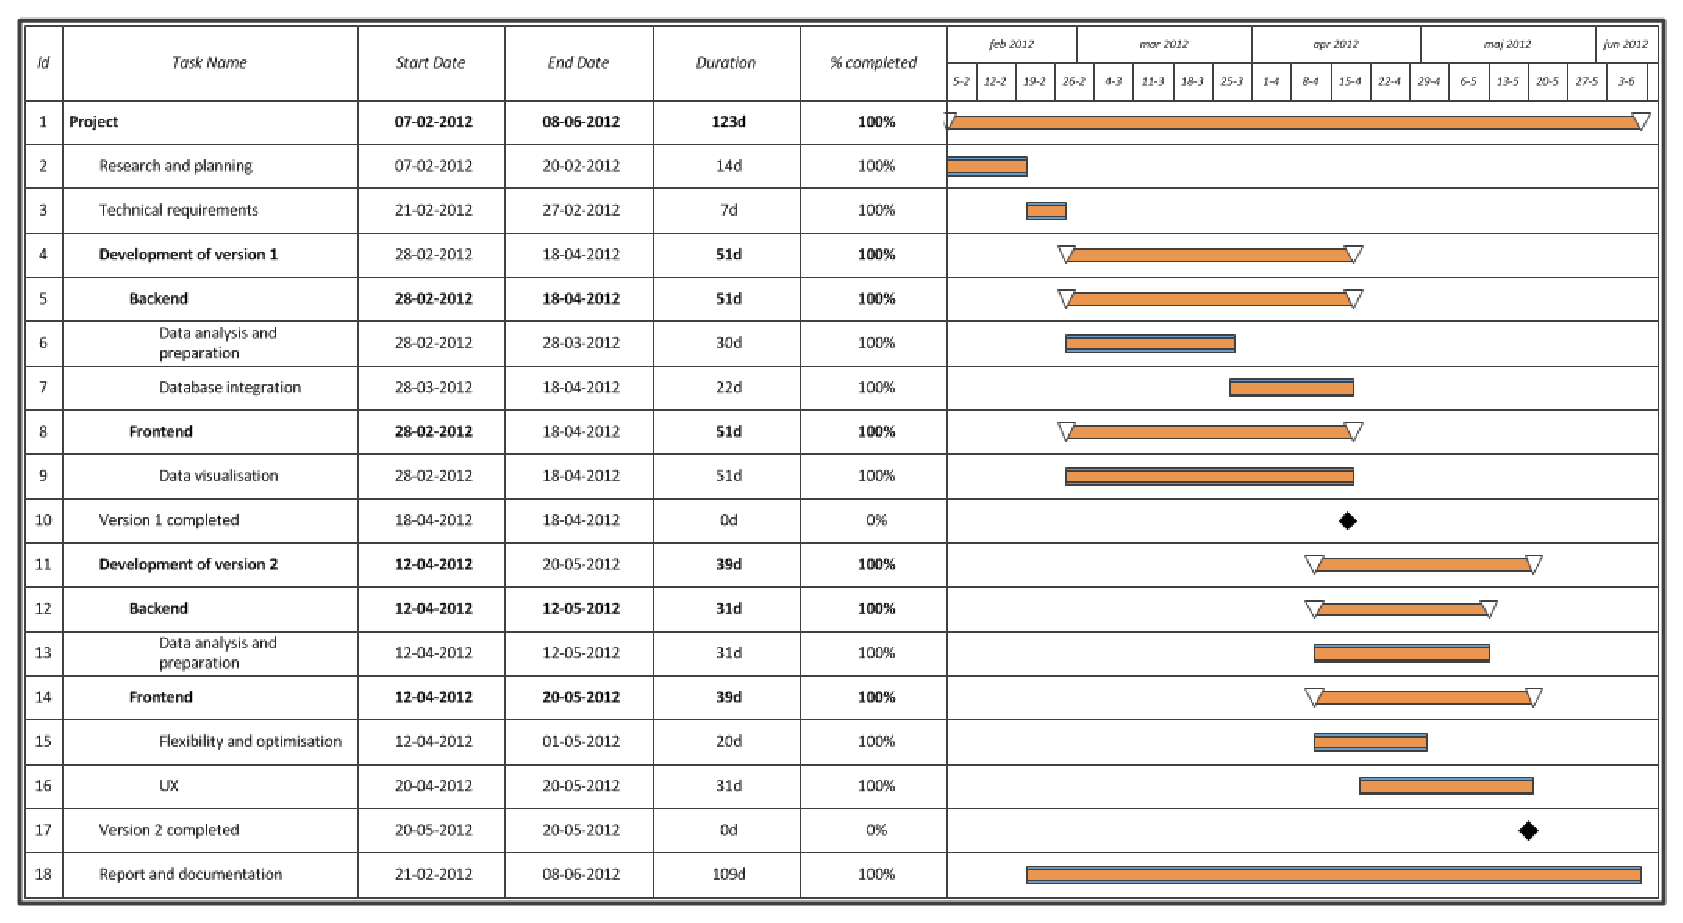
\includegraphics[height=.65\linewidth,angle=90]{figure/planning2.eps}
\end{figure}